%=========================
% Sections/03-CongTrinhLienQuan.tex
% Chương 3 – Các công trình liên quan
%=========================
\section{Công nghệ liên quan}
\subsection{Kiến trúc hệ thống AI}

Kiến trúc hệ thống là một trong những yếu tố quan trọng quyết định khả năng mở rộng, hiệu năng và tính linh hoạt của hệ thống phần mềm. Kiến trúc phần mềm mô tả cấu trúc tổng thể của hệ thống, bao gồm các thành phần chính, mối quan hệ giữa các thành phần và cách chúng tương tác với nhau trong quá trình xử lý dữ liệu.

Trong các hệ thống hiện đại, đặc biệt là hệ thống trí tuệ nhân tạo trong lĩnh vực thương mại điện tử, kiến trúc hệ thống cần hỗ trợ xử lý phân tán, tích hợp nhiều dịch vụ AI và đảm bảo khả năng mở rộng linh hoạt theo tải hệ thống. Các mô hình kiến trúc phổ biến hiện nay bao gồm monolithic architecture, microservice architecture và cloud-native architecture.

%=========================
\subsubsection{Monolithic Architecture}

Monolithic architecture là mô hình kiến trúc trong đó toàn bộ hệ thống được xây dựng và triển khai như một khối thống nhất. Các thành phần như giao diện người dùng, logic nghiệp vụ và tầng truy cập dữ liệu thường nằm trong cùng một ứng dụng, chia sẻ chung mã nguồn, môi trường chạy và quy trình triển khai.

Như trình bày ở \Cref{fig:monolithic_architecture}, toàn bộ hệ thống được triển khai trong một khối thống nhất.

\begin{figure}[H]
    \centering
    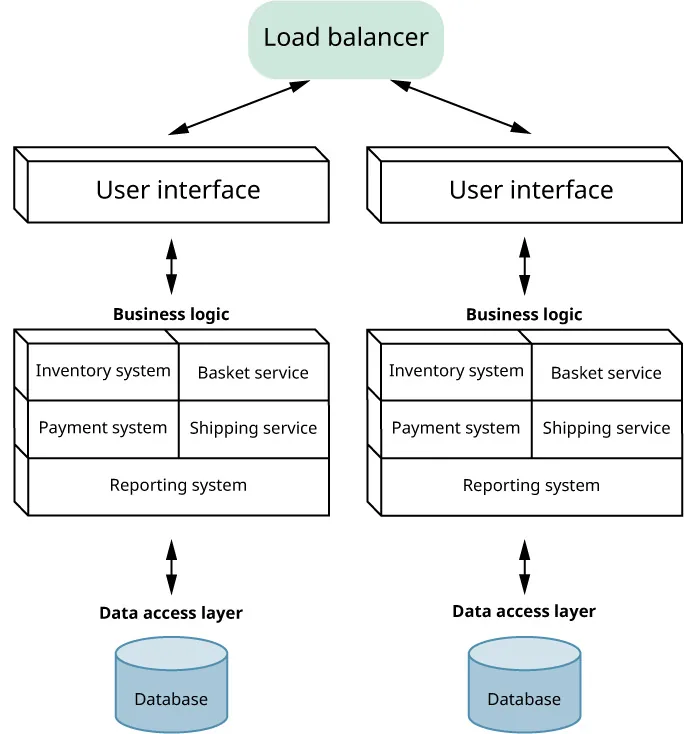
\includegraphics[width=0.5\textwidth]{Images/Congnghelienquan/Monolithic_architecture.png}
    \caption{Kiến trúc monolithic trong đó toàn bộ thành phần hệ thống được triển khai trong một ứng dụng duy nhất (nguồn: OpenStax \parencite{openstax_cloud_native_intro})}
    \label{fig:monolithic_architecture}
\end{figure}

Trong kiến trúc monolithic, toàn bộ hệ thống thường nằm trong một codebase duy nhất, các module chia sẻ chung tài nguyên và giao tiếp nội bộ trong cùng tiến trình. Cách tổ chức này giúp việc phát triển, kiểm thử và triển khai ban đầu trở nên đơn giản, đặc biệt phù hợp với các hệ thống nhỏ hoặc các phiên bản thử nghiệm ban đầu.

Ưu điểm của monolithic architecture là cấu trúc dễ hiểu, ít phức tạp trong triển khai và có hiệu năng tốt do không phát sinh overhead mạng giữa các thành phần. Tuy nhiên, khi hệ thống phát triển lớn hơn, kiến trúc này có thể gặp khó khăn trong việc mở rộng, bảo trì và cập nhật từng chức năng riêng lẻ. Sự phụ thuộc chặt giữa các module cũng khiến việc thay đổi một thành phần có thể ảnh hưởng đến toàn bộ hệ thống.

%=========================
\subsubsection{Microservice Architecture}

Microservice architecture là mô hình kiến trúc trong đó hệ thống được chia thành nhiều dịch vụ nhỏ, độc lập và giao tiếp với nhau thông qua API. Mỗi service thường đảm nhiệm một chức năng nghiệp vụ riêng, có thể được phát triển, kiểm thử, triển khai và mở rộng độc lập với các service khác.

Như trình bày ở \Cref{fig:microservice_architecture}, hệ thống được phân tách thành các service độc lập.

\begin{figure}[H]
    \centering
    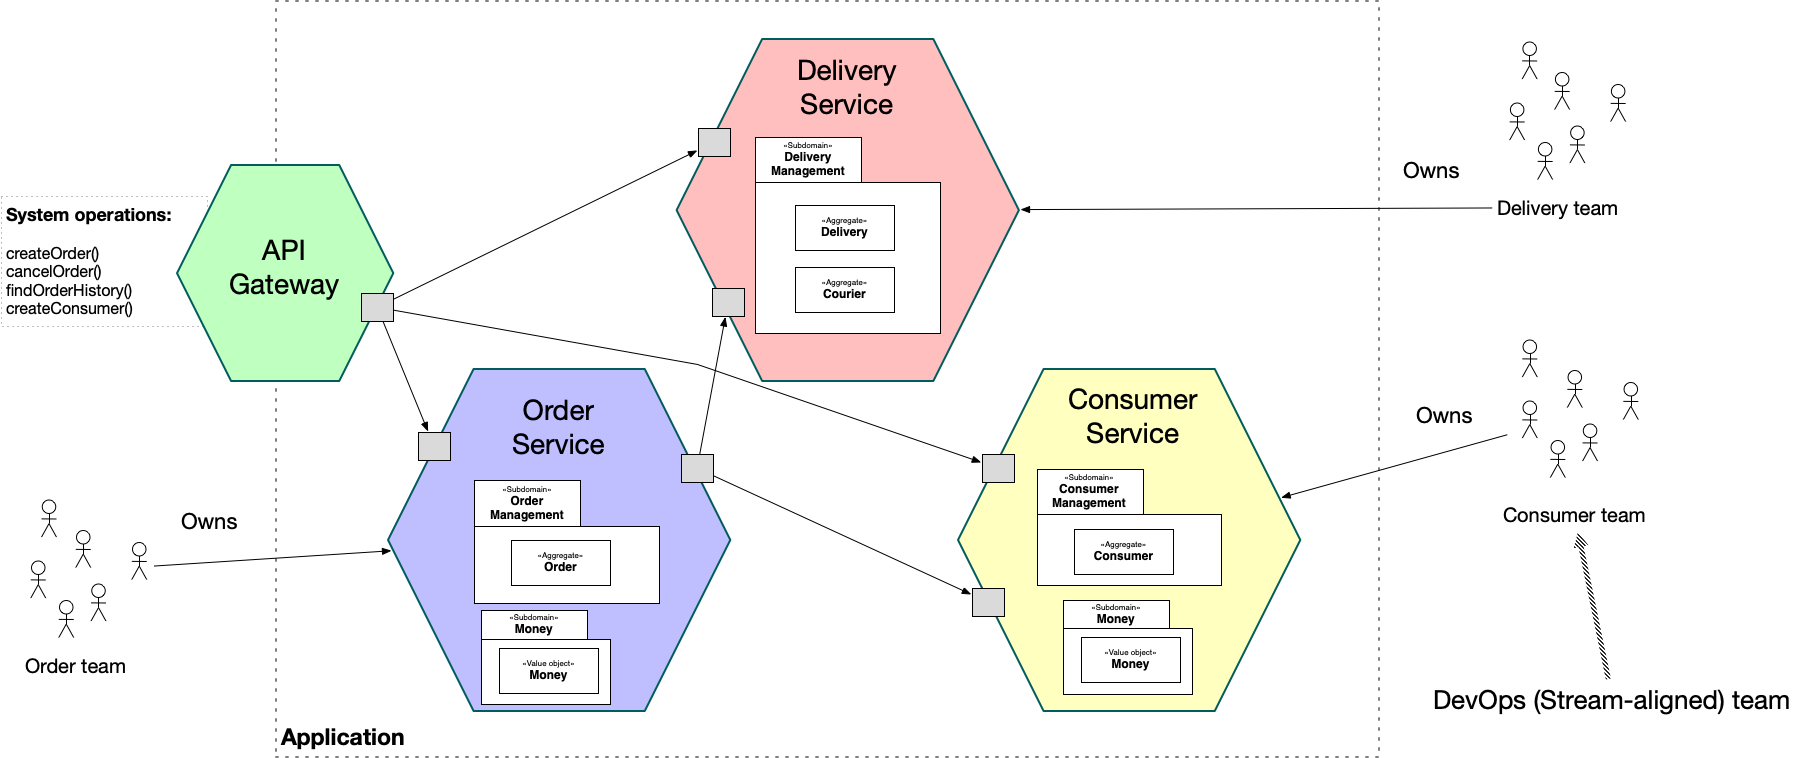
\includegraphics[width=0.85\textwidth]{Images/Congnghelienquan/microservices-teams-subdomains.png}
    \caption{Kiến trúc microservice trong đó hệ thống được chia thành các dịch vụ nhỏ, độc lập và giao tiếp qua API (nguồn: Microservices.io \parencite{microservices_io_patterns})}
    \label{fig:microservice_architecture}
\end{figure}

Trong kiến trúc microservice, hệ thống được tổ chức thành nhiều service độc lập, mỗi service phụ trách một nhóm chức năng cụ thể và giao tiếp với nhau thông qua REST API, gRPC hoặc message broker. Các service có thể được phát triển bằng công nghệ khác nhau tùy theo yêu cầu nghiệp vụ, miễn là chúng tuân thủ cơ chế giao tiếp đã được thiết kế.

Ưu điểm của microservice architecture là khả năng mở rộng linh hoạt theo từng thành phần, hỗ trợ phát triển song song giữa các nhóm và tăng khả năng chịu lỗi của hệ thống. Khi một service gặp sự cố, các service khác vẫn có thể tiếp tục hoạt động nếu hệ thống được thiết kế tốt.

Tuy nhiên, microservice cũng làm tăng độ phức tạp trong vận hành vì hệ thống trở thành một môi trường phân tán. Việc triển khai, monitoring, logging, tracing và orchestration cần được quản lý chặt chẽ. Ngoài ra, giao tiếp giữa các service có thể phát sinh overhead mạng và làm tăng độ trễ so với kiến trúc monolithic.
%=========================
\subsubsection{Service-based Architecture}

Service-based architecture là mô hình kiến trúc trong đó hệ thống được chia thành nhiều service độc lập theo từng nhóm chức năng hoặc nghiệp vụ. Mỗi service đảm nhiệm một vai trò cụ thể và giao tiếp với các service khác thông qua API. Cách tiếp cận này giúp hệ thống dễ mở rộng, dễ bảo trì và phù hợp với các hệ thống có nhiều thành phần xử lý riêng biệt như tìm kiếm, gợi ý sản phẩm, quản lý người dùng và xử lý AI.

Khác với monolithic architecture, service-based architecture không gom toàn bộ chức năng vào một ứng dụng duy nhất. Thay vào đó, hệ thống được tổ chức thành các service có trách nhiệm rõ ràng. Tuy nhiên, mô hình này không nhất thiết phải tách nhỏ đến mức microservices hoàn chỉnh, mà có thể chia theo các module lớn hơn để giảm độ phức tạp trong triển khai.

Như trình bày ở \Cref{fig:service_based_architecture}, hệ thống service-based được tổ chức thành nhiều service độc lập và giao tiếp với nhau thông qua API.

\begin{figure}[H]
    \centering
    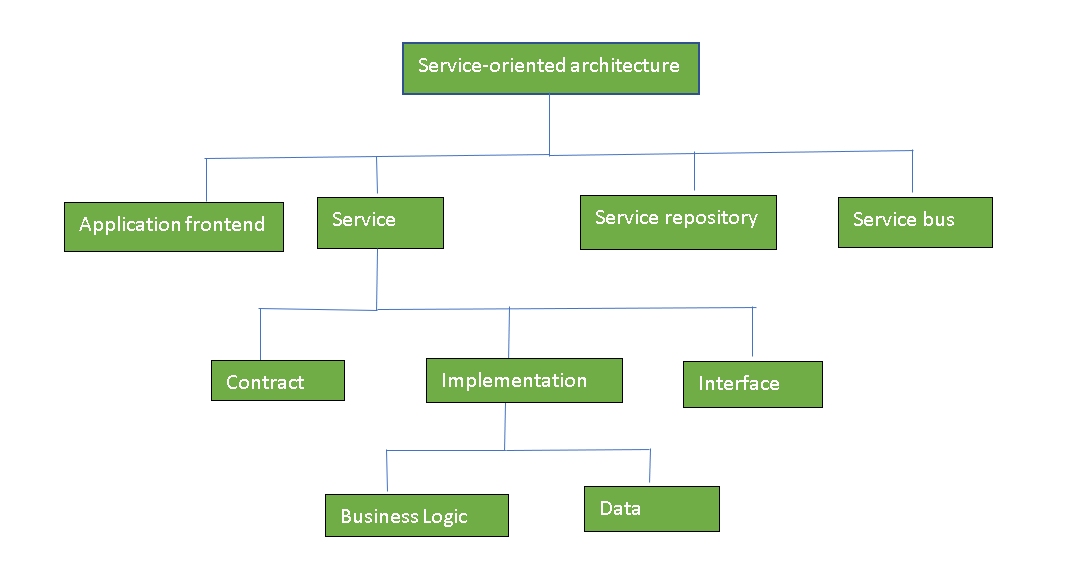
\includegraphics[width=0.85\textwidth]{Images/Congnghelienquan/service-base-architectural.png}
    \caption{Kiến trúc service-based chia hệ thống thành nhiều service độc lập và giao tiếp thông qua API \parencite{geeksforgeeks2023soa}}
    \label{fig:service_based_architecture}
\end{figure}

Trong service-based architecture, hệ thống được chia thành các service theo chức năng, mỗi service có thể được phát triển, bảo trì và mở rộng tương đối độc lập. Các service giao tiếp với nhau thông qua API, giúp giảm sự phụ thuộc trực tiếp giữa các module so với monolithic architecture.

Ưu điểm của kiến trúc này là dễ mở rộng từng thành phần, dễ thay đổi hoặc nâng cấp một service mà không ảnh hưởng quá nhiều đến toàn bộ hệ thống. Mô hình này cũng phù hợp với các hệ thống có nhiều thành phần riêng biệt như search service, recommendation service, user service, LLM service và vector database service.

Tuy nhiên, service-based architecture yêu cầu thiết kế API rõ ràng giữa các service. Việc quản lý giao tiếp, đồng bộ dữ liệu và xử lý lỗi giữa các service cũng phức tạp hơn so với monolithic architecture. Ngoài ra, hệ thống có thể phát sinh độ trễ khi các service gọi nhau thông qua mạng.

%=========================
\subsubsection{So sánh kiến trúc hệ thống}

Như tổng hợp ở Bảng \Cref{tab:architecture_comparison}, các kiến trúc được so sánh dựa trên khả năng mở rộng, mức độ triển khai, bảo trì và sự phù hợp với hệ thống AI.

\begin{table}[H]
\centering
\caption{So sánh các kiến trúc hệ thống phổ biến trong ứng dụng AI hiện đại}
\label{tab:architecture_comparison}
\renewcommand{\arraystretch}{1.3}

\begin{tabular}{@{}lccc@{}}
\toprule
\textbf{Tiêu chí} & \textbf{Monolithic} & \textbf{Microservice} & \textbf{Service-based} \\
\midrule
Khả năng mở rộng & Thấp & Cao & Rất cao \\
Triển khai & Đơn giản & Trung bình & Phức tạp \\
Bảo trì & Khó & Dễ & Dễ hơn monolithic \\
Hiệu năng & Tốt (nhỏ) & Ổn định & Tối ưu cho các service lớn \\
Phù hợp AI system & Thấp & Cao & Rất cao \\
\bottomrule
\end{tabular}
\end{table}

Tổng kết lại, kiến trúc microservice và service-based là lựa chọn phù hợp cho các hệ thống AI hiện đại nhờ khả năng mở rộng linh hoạt, hỗ trợ triển khai phân tán và tích hợp tốt với các thành phần như vector database, embedding models và các dịch vụ AI.
%=========================
\subsection{Backend Framework}
\subsubsection{Spring Boot}

Spring Boot là framework phát triển ứng dụng backend dựa trên Spring Framework, được thiết kế nhằm đơn giản hóa quá trình xây dựng và triển khai ứng dụng Java enterprise \parencite{springbootdocs2024}. Framework cung cấp cơ chế auto-configuration, dependency management và embedded server giúp giảm đáng kể khối lượng cấu hình thủ công trong quá trình phát triển hệ thống.

Spring Boot hỗ trợ xây dựng các ứng dụng theo kiến trúc RESTful API và microservices, đồng thời tích hợp tốt với nhiều công nghệ backend hiện đại như ORM, security framework và message broker. Nhờ hệ sinh thái mạnh mẽ của Spring, framework này được sử dụng rộng rãi trong các hệ thống enterprise yêu cầu độ ổn định và khả năng mở rộng cao.

Trong hệ thống AI Shopping Assistant, Spring Boot được sử dụng làm nền tảng backend chính nhằm xử lý business logic, quản lý API và điều phối các dịch vụ trong hệ thống.

\textbf{Ứng dụng trong hệ thống:}
\begin{itemize}
    \item Xây dựng RESTful API cho hệ thống E-commerce
    
    \item Quản lý xác thực và phân quyền người dùng
    
    \item Kết nối và thao tác với cơ sở dữ liệu quan hệ
    
    \item Điều phối nghiệp vụ giữa các service
\end{itemize}

%=========================

\subsubsection{FastAPI}

FastAPI là framework backend dành cho Python được phát triển nhằm hỗ trợ xây dựng API hiệu năng cao và hỗ trợ lập trình bất đồng bộ \parencite{fastapidocs2024}. Framework được xây dựng dựa trên chuẩn ASGI và tận dụng Python type hints để hỗ trợ kiểm tra dữ liệu đầu vào cũng như tự động sinh tài liệu API theo chuẩn OpenAPI.

FastAPI có khả năng xử lý request với hiệu năng cao, đồng thời tích hợp tốt với các thư viện AI và machine learning phổ biến như PyTorch, TensorFlow và HuggingFace. Điều này giúp framework trở thành lựa chọn phù hợp cho các hệ thống trí tuệ nhân tạo và xử lý dữ liệu phi cấu trúc.

Trong hệ thống AI Shopping Assistant, FastAPI được sử dụng chủ yếu cho các AI service và các thành phần liên quan đến retrieval pipeline.

\textbf{Ứng dụng trong hệ thống:}
\begin{itemize}
    \item Triển khai embedding service và vector retrieval
    
    \item Tích hợp Large Language Model phục vụ inference
    
    \item Xây dựng RAG pipeline
    
    \item Xử lý Computer Vision và NLP service
\end{itemize}

%=========================

\subsubsection{Node.js}

Node.js là môi trường runtime JavaScript được xây dựng trên V8 engine của Google Chrome nhằm hỗ trợ phát triển ứng dụng phía server \parencite{nodejsdocs2024}. Node.js sử dụng mô hình event-driven và non-blocking I/O giúp tối ưu khả năng xử lý đồng thời và giảm chi phí tài nguyên trong các hệ thống có lượng request lớn.

Khác với các kiến trúc xử lý đồng bộ truyền thống, Node.js cho phép hệ thống xử lý nhiều kết nối đồng thời thông qua cơ chế asynchronous programming. Điều này giúp Node.js phù hợp với các ứng dụng realtime hoặc các dịch vụ cần phản hồi nhanh.

Trong các hệ thống backend hiện đại, Node.js thường được sử dụng cho các thành phần realtime hoặc lightweight service.

\textbf{Ứng dụng trong hệ thống:}
\begin{itemize}
    \item Xử lý giao tiếp realtime
    
    \item Xây dựng notification service
    
    \item Triển khai API Gateway hoặc Backend for Frontend
    
    \item Hỗ trợ streaming và event processing
\end{itemize}

%=========================
\subsubsection{So sánh Backend Framework}

Nhằm làm rõ sự khác biệt giữa các backend framework, Bảng \Cref{tab:backend_framework} tổng hợp so sánh dựa trên các tiêu chí quan trọng như hiệu năng, khả năng hỗ trợ AI và mức độ phù hợp với hệ thống phân tán.

\begin{table}[H]
\centering
\caption{So sánh các backend framework phổ biến dựa trên hiệu năng, khả năng hỗ trợ AI và mức độ phù hợp với kiến trúc hệ thống phân tán}
\label{tab:backend_framework}
\renewcommand{\arraystretch}{1.3}

\begin{tabular}{@{}lccc@{}}
\toprule
\textbf{Tiêu chí} & \textbf{Spring Boot} & \textbf{FastAPI} & \textbf{Node.js} \\
\midrule
Ngôn ngữ & Java & Python & JavaScript \\
Hiệu năng & Cao & Rất cao & Cao \\
Hỗ trợ AI/ML & Trung bình & Rất tốt & Thấp \\
Microservices & Rất tốt & Tốt & Tốt \\
Realtime & Tốt & Trung bình & Rất tốt \\
Ứng dụng phù hợp & Enterprise backend & AI services & Realtime systems \\
\bottomrule
\end{tabular}
\end{table}

Trong hệ thống AI Shopping Assistant, việc kết hợp nhiều backend framework cho phép tận dụng ưu điểm riêng của từng công nghệ trong từng lớp kiến trúc.

Cụ thể:
\begin{itemize}
    \item Spring Boot đảm nhận vai trò backend core và xử lý business logic
    \item FastAPI phụ trách các AI services và inference pipeline
    \item Node.js đảm nhận lớp realtime và giao tiếp thời gian thực
\end{itemize}

Mô hình backend đa framework này giúp hệ thống đạt được khả năng mở rộng linh hoạt, tối ưu hiệu năng theo từng loại tác vụ và tách biệt rõ ràng giữa AI services và business logic.
\subsection{Frontend Framework}

Frontend framework đóng vai trò quan trọng trong việc xây dựng UI , đảm bảo UX , khả năng tương tác và hiệu năng hiển thị của hệ thống. Trong các hệ thống hiện đại như AI Shopping Assistant, frontend không chỉ đảm nhiệm việc hiển thị dữ liệu mà còn hỗ trợ tìm kiếm thông minh, cập nhật realtime và tương tác đa phương tiện với backend và AI services.

%=========================
\subsubsection{React}

React là một thư viện JavaScript do Meta phát triển, được thiết kế theo kiến trúc component-based \textcite{reactdocs2024}. React sử dụng Virtual DOM nhằm tối ưu hiệu năng khi cập nhật giao diện người dùng.

Trong hệ thống AI Shopping Assistant, React đóng vai trò là framework frontend chính, chịu trách nhiệm xây dựng giao diện web và quản lý tương tác người dùng.

Như trình bày ở các ứng dụng web hiện đại, React đặc biệt phù hợp với các hệ thống có dữ liệu động và yêu cầu cập nhật giao diện theo thời gian thực.

\textbf{Ứng dụng trong hệ thống:}
\begin{itemize}
    \item Xây dựng giao diện web thương mại điện tử
    \item Hiển thị kết quả tìm kiếm AI (text, image, ranking)
    \item Quản lý trạng thái người dùng (cart, session, history)
    \item Tích hợp API từ backend và AI services
\end{itemize}

React có ưu điểm về tính linh hoạt cao, hệ sinh thái lớn và khả năng mở rộng tốt cho các ứng dụng web hiện đại.

%=========================
\subsubsection{Angular}

Angular là framework frontend toàn diện do Google phát triển, dựa trên TypeScript \textcite{angulardocs2024}. Framework này cung cấp sẵn các thành phần như routing, form handling, dependency injection và state management.

Angular thường được sử dụng trong các hệ thống doanh nghiệp có độ phức tạp cao và yêu cầu kiến trúc chặt chẽ.

\textbf{Ứng dụng trong thực tế:}
\begin{itemize}
    \item Ứng dụng doanh nghiệp lớn (enterprise applications)
    \item Hệ thống dashboard và admin panel phức tạp
    \item Các hệ thống yêu cầu kiến trúc chuẩn hóa cao
\end{itemize}

Angular có ưu điểm về kiến trúc rõ ràng và tính nhất quán cao, tuy nhiên độ phức tạp lớn hơn so với React.

%=========================
\subsubsection{Vue}

Vue.js là framework frontend nhẹ, linh hoạt và dễ tiếp cận \textcite{vuedocs2024}. Vue kết hợp ưu điểm của React  và Angular , nhưng đơn giản hơn trong quá trình triển khai.

Vue thường được sử dụng trong các dự án có yêu cầu phát triển nhanh hoặc quy mô nhỏ đến trung bình.

\textbf{Ứng dụng trong thực tế:}
\begin{itemize}
    \item Website thương mại điện tử nhỏ và vừa
    \item Prototype hoặc MVP development
    \item Ứng dụng cần phát triển nhanh
\end{itemize}

Vue phù hợp với nhóm phát triển nhỏ nhờ cú pháp đơn giản và khả năng học nhanh.

%=========================
\subsubsection{So sánh frontend framework}

Nhằm làm rõ sự khác biệt giữa các frontend framework, Bảng \Cref{tab:frontend_framework_comparison} tổng hợp so sánh dựa trên các tiêu chí như hiệu năng, độ phức tạp và mức độ phù hợp với hệ thống AI.

\begin{table}[H]
\centering
\caption{So sánh các frontend framework phổ biến dựa trên kiến trúc, hiệu năng và mức độ phù hợp với hệ thống AI hiện đại}
\label{tab:frontend_framework_comparison}
\renewcommand{\arraystretch}{1.3}

\begin{tabular}{@{}lccc@{}}
\toprule
\textbf{Tiêu chí} & \textbf{React} & \textbf{Angular} & \textbf{Vue} \\
\midrule
Loại & Library & Full framework & Progressive framework \\
Ngôn ngữ & JavaScript/JSX & TypeScript & JavaScript \\
Hiệu năng & Cao & Cao & Cao \\
Độ phức tạp & Trung bình & Cao & Thấp \\
Hệ sinh thái & Rất lớn & Lớn & Trung bình \\
Độ linh hoạt & Rất cao & Trung bình & Cao \\
Phù hợp AI system & Rất tốt & Tốt & Trung bình \\
\bottomrule
\end{tabular}
\end{table}

Trong hệ thống AI Shopping Assistant, React được lựa chọn làm frontend chính nhờ khả năng linh hoạt cao, hỗ trợ tốt cho giao diện động và khả năng tích hợp dễ dàng với các API AI cũng như dữ liệu realtime từ backend services.
\subsection{Embedding Models}

Embedding models được sử dụng để biểu diễn dữ liệu như văn bản và hình ảnh dưới dạng vector embedding phục vụ semantic search và multimodal retrieval.

Trong hệ thống AI Shopping Assistant, embedding models hỗ trợ tìm kiếm sản phẩm, visual search và tăng hiệu quả retrieval trong kiến trúc RAG.
%=========================
\subsubsection{BERT-based Models}

BERT là mô hình ngôn ngữ được Google giới thiệu vào năm 2018, dựa trên kiến trúc Transformer Encoder \textcite{devlin2018bert}. Khác với các mô hình ngôn ngữ truyền thống thường xử lý văn bản theo một chiều, BERT học biểu diễn ngữ cảnh hai chiều, giúp mô hình hiểu tốt hơn mối quan hệ giữa các từ trong câu.

BERT sử dụng cơ chế self-attention để mô hình hóa quan hệ giữa các token trong chuỗi đầu vào. Nhờ đó, mô hình có thể tạo ra biểu diễn ngữ nghĩa giàu thông tin, phù hợp cho nhiều tác vụ xử lý ngôn ngữ tự nhiên và truy xuất thông tin.

Trong hệ thống AI Shopping Assistant, BERT-based models có thể được sử dụng để mã hóa truy vấn người dùng, biểu diễn mô tả sản phẩm, hỗ trợ semantic search, query understanding, intent detection và retrieval trong RAG pipeline. Các biến thể phổ biến của BERT trong bài toán embedding gồm Sentence-BERT, MiniLM, MPNet và E5 models.

Ưu điểm của BERT-based models là khả năng hiểu ngữ cảnh tốt, biểu diễn ngữ nghĩa mạnh và hiệu quả trong các bài toán retrieval trên dữ liệu văn bản. Tuy nhiên, các mô hình này thường có chi phí tính toán cao hơn so với các mô hình nhẹ, không xử lý trực tiếp dữ liệu hình ảnh và còn hạn chế trong các bài toán đa phương thức nếu không được kết hợp với mô hình thị giác.

\begin{figure}[H]
    \centering
    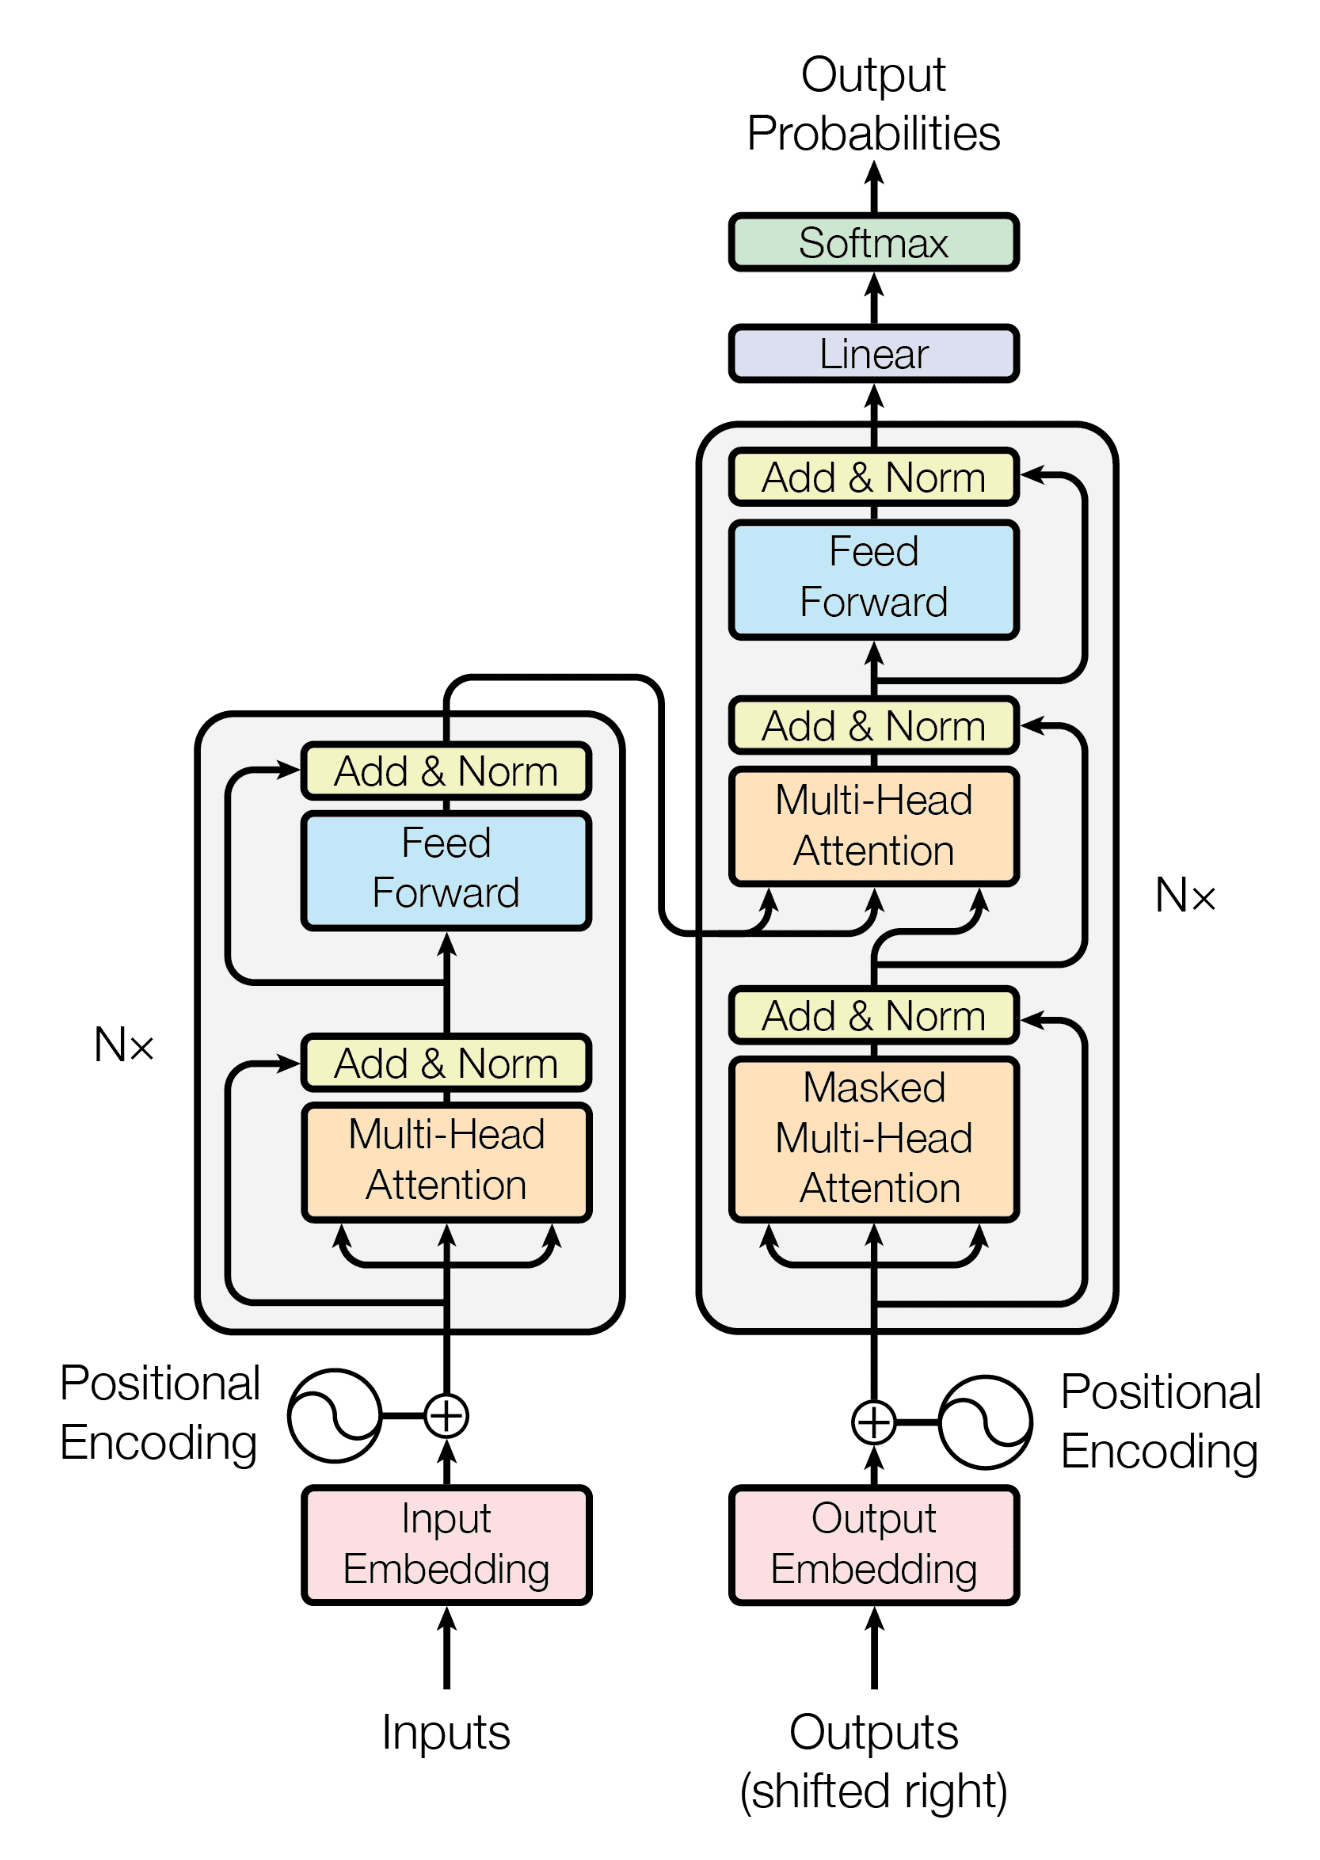
\includegraphics[width=0.6\textwidth]{Images/Congnghelienquan/attention_research_1.png}
    \caption{Kiến trúc Transformer Encoder trong mô hình BERT \parencite{viblo_transformer_bert}}
    \label{fig:bert_transformer}
\end{figure}

Hình \Cref{fig:bert_transformer} minh họa kiến trúc Transformer Encoder được sử dụng trong BERT, trong đó cơ chế self-attention đóng vai trò cốt lõi trong việc học biểu diễn ngữ cảnh.
%=========================
\subsubsection{CLIP}

CLIP là mô hình học đa phương thức do OpenAI phát triển, nhằm xây dựng một không gian embedding chung cho cả hình ảnh và văn bản \textcite{radford2021clip}. Mô hình này được huấn luyện trên tập dữ liệu lớn gồm các cặp image-text bằng phương pháp contrastive learning, giúp hệ thống học được mối liên hệ ngữ nghĩa giữa nội dung hình ảnh và mô tả văn bản tương ứng.

Kiến trúc của CLIP gồm hai encoder độc lập: image encoder dùng để mã hóa hình ảnh và text encoder dùng để mã hóa văn bản. Image encoder có thể được xây dựng dựa trên CNN hoặc Vision Transformer, trong khi text encoder thường dựa trên kiến trúc Transformer. Hai encoder này ánh xạ hình ảnh và văn bản vào cùng một embedding space, trong đó các cặp image-text liên quan sẽ có vector gần nhau, còn các cặp không liên quan sẽ có vector xa nhau.

Cách tiếp cận này giúp CLIP có khả năng zero-shot learning mạnh và hỗ trợ tốt các bài toán truy xuất đa phương thức như text-to-image retrieval, image-to-image search, cross-modal search và multimodal recommendation.

\begin{figure}[H]
    \centering
    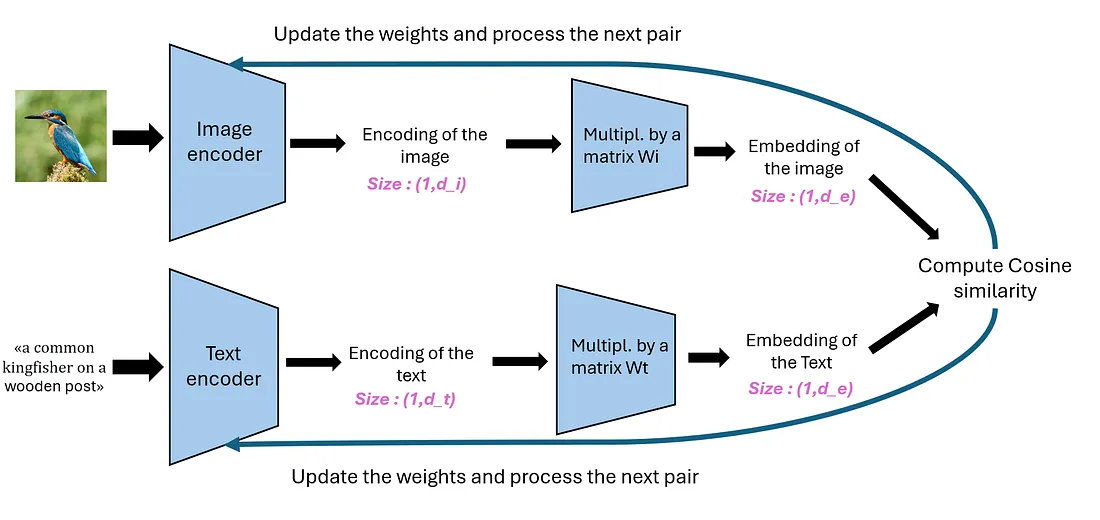
\includegraphics[width=0.85\textwidth]{Images/Congnghelienquan/clip_architecture.png}
    \caption{Kiến trúc tổng quát của mô hình CLIP với dual-encoder gồm image encoder và text encoder ánh xạ vào cùng một không gian embedding chung (nguồn: Medium \parencite{medium_clip_multimodal_embedding})}
    \label{fig:clip_architecture}
\end{figure}

Hình \Cref{fig:clip_architecture} mô tả kiến trúc dual-encoder của CLIP, trong đó hình ảnh và văn bản được mã hóa riêng biệt nhưng được biểu diễn trong cùng một không gian embedding. Nhờ đó, hệ thống có thể so sánh trực tiếp độ tương đồng giữa truy vấn văn bản và hình ảnh sản phẩm.

Trong hệ thống AI Shopping Assistant, CLIP có thể được sử dụng cho các bài toán truy xuất đa phương thức như tìm kiếm sản phẩm bằng hình ảnh, tìm ảnh sản phẩm theo mô tả văn bản, gợi ý sản phẩm tương tự và kết nối dữ liệu văn bản với dữ liệu hình ảnh. Ví dụ, khi người dùng nhập truy vấn ``áo khoác màu đen phong cách thể thao'', hệ thống có thể dùng text embedding của truy vấn để tìm các hình ảnh sản phẩm có đặc trưng thị giác tương ứng.

Ưu điểm của CLIP là khả năng biểu diễn hình ảnh và văn bản trong cùng một không gian ngữ nghĩa, hiệu quả cao trong semantic visual search và có khả năng zero-shot tốt. Tuy nhiên, mô hình này có chi phí huấn luyện và suy luận tương đối cao, yêu cầu tài nguyên GPU lớn và có thể chịu ảnh hưởng bởi bias từ dữ liệu huấn luyện trên Internet.

CLIP hiện là một trong những nền tảng quan trọng trong các hệ thống trí tuệ nhân tạo đa phương thức hiện đại, đặc biệt trong các bài toán kết hợp giữa ngôn ngữ tự nhiên và dữ liệu hình ảnh.
%=========================
\subsubsection{SigLIP}

SigLIP là mô hình học đa phương thức do Google Research phát triển nhằm cải tiến cơ chế huấn luyện so với CLIP \cite{zhai2023siglip}. Thay vì sử dụng softmax contrastive loss như CLIP, SigLIP áp dụng sigmoid loss độc lập cho từng cặp image-text. Cách tiếp cận này giúp đơn giản hóa quá trình tối ưu hóa, giảm sự phụ thuộc vào batch size lớn và hỗ trợ huấn luyện hiệu quả hơn trên tập dữ liệu quy mô lớn.

Kiến trúc của SigLIP vẫn dựa trên mô hình dual-encoder, gồm image encoder và text encoder hoạt động độc lập. Trong đó, image encoder thường sử dụng Vision Transformer (ViT) để mã hóa hình ảnh, còn text encoder dựa trên kiến trúc Transformer để mã hóa văn bản. Hai encoder này ánh xạ dữ liệu hình ảnh và văn bản vào cùng một không gian embedding, giúp hệ thống đo được mức độ tương đồng giữa nội dung thị giác và mô tả ngôn ngữ.

\begin{figure}[H]
    \centering
    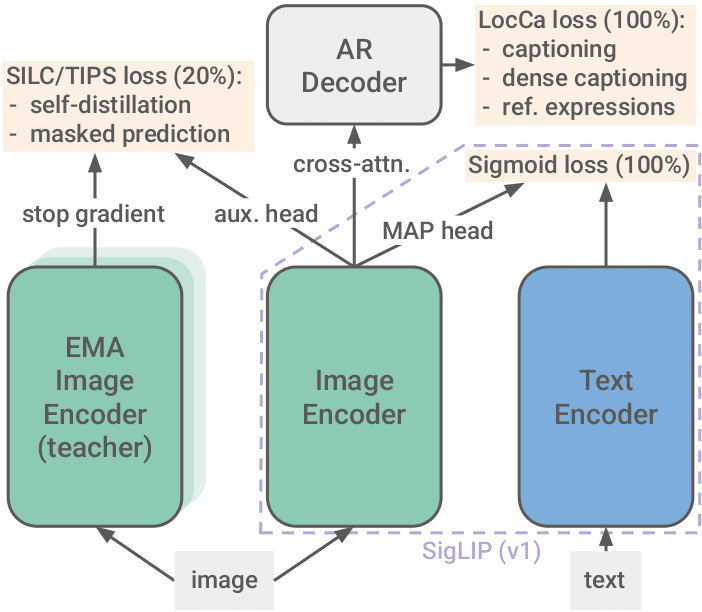
\includegraphics[width=0.6\textwidth]{Images/Congnghelienquan/siglip_architecture1.png}
    \caption{Kiến trúc dual-encoder của mô hình SigLIP với cơ chế sigmoid loss cho huấn luyện đa phương thức (nguồn: LearnOpenCV \parencite{learnopencv_siglip2})}
    \label{fig:siglip_architecture}
\end{figure}

Hình \Cref{fig:siglip_architecture} minh họa kiến trúc dual-encoder của SigLIP, trong đó hình ảnh và văn bản được mã hóa riêng biệt nhưng được đưa về cùng một không gian biểu diễn. Nhờ cơ chế sigmoid loss, SigLIP có thể học quan hệ giữa các cặp image-text theo cách linh hoạt hơn, đặc biệt trong bối cảnh huấn luyện với dữ liệu lớn.

Trong các benchmark về retrieval và zero-shot classification, SigLIP cho thấy hiệu năng cạnh tranh hoặc vượt CLIP trong nhiều kịch bản. Điều này giúp SigLIP trở thành một lựa chọn phù hợp cho các bài toán cần biểu diễn đa phương thức chất lượng cao.

Trong hệ thống AI Shopping Assistant, SigLIP có thể được sử dụng cho visual product retrieval, multimodal semantic search, similar item recommendation và fashion-aware visual search. Ví dụ, hệ thống có thể dùng SigLIP để ánh xạ ảnh sản phẩm và truy vấn văn bản vào cùng một không gian embedding, từ đó tìm ra các sản phẩm có đặc điểm hình ảnh hoặc phong cách gần với nhu cầu của người dùng.

%=========================
\subsubsection{ViT}

Vision Transformer (ViT) là mô hình áp dụng kiến trúc Transformer vào bài toán thị giác máy tính, được giới thiệu bởi Google Research năm 2020 \textcite{dosovitskiy2020vit}. Khác với CNN truyền thống dựa trên phép tích chập, ViT xử lý hình ảnh như một chuỗi các patch, tương tự cách mô hình ngôn ngữ xử lý chuỗi token trong NLP.

Trong ViT, ảnh đầu vào được chia thành các patch có kích thước cố định. Mỗi patch sau đó được chuyển thành vector embedding và kết hợp với positional embedding để giữ lại thông tin vị trí trong ảnh. Chuỗi embedding này được đưa vào Transformer Encoder để học mối quan hệ giữa các vùng ảnh và tạo ra image embedding đầu ra.

Cơ chế self-attention giúp ViT học được quan hệ toàn cục giữa các vùng trong ảnh, thay vì chỉ tập trung vào các đặc trưng cục bộ như CNN. Nhờ đó, ViT có khả năng biểu diễn hình ảnh hiệu quả trong nhiều bài toán như image classification, visual retrieval và multimodal learning.

\begin{figure}[H]
    \centering
    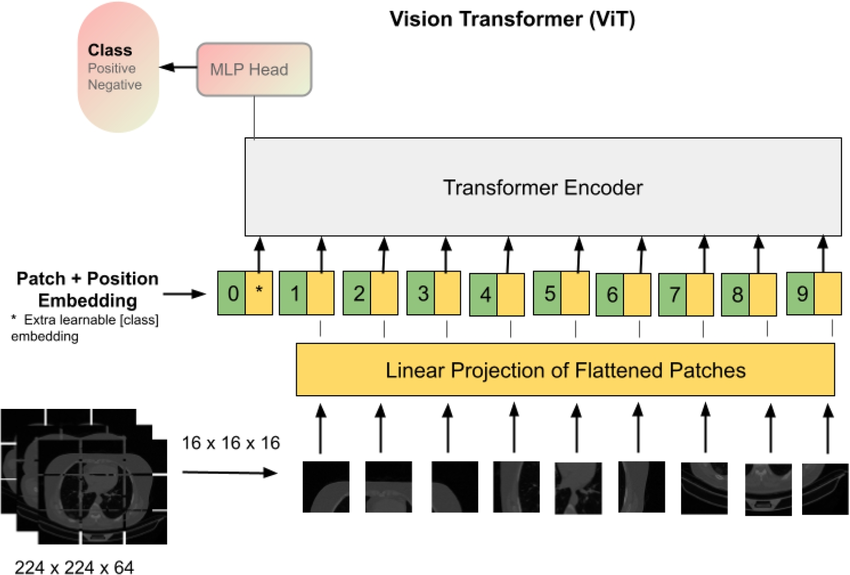
\includegraphics[width=0.75\textwidth]{Images/Congnghelienquan/vit_architecture.png}
    \caption{Kiến trúc Vision Transformer với cách biểu diễn ảnh dưới dạng chuỗi patch, trong đó ảnh được chia thành các patch không chồng lấp và ánh xạ thành embedding trước khi đưa vào Transformer encoder (nguồn: ResearchGate \parencite{researchgate_vit_patch_architecture})}
    \label{fig:vit_architecture}
\end{figure}

Hình \Cref{fig:vit_architecture} mô tả cách ViT chuyển ảnh thành chuỗi patch trước khi đưa vào Transformer Encoder. Quá trình này giúp mô hình xử lý ảnh theo dạng tuần tự và tận dụng cơ chế attention để học quan hệ giữa các phần khác nhau của hình ảnh.

Trong hệ thống AI Shopping Assistant, ViT có thể được sử dụng để trích xuất image embedding cho sản phẩm, hỗ trợ visual search và phục vụ image retrieval trong vector database. Ngoài ra, ViT còn đóng vai trò là backbone quan trọng trong nhiều mô hình multimodal như CLIP và SigLIP.
\subsubsection{So sánh Embedding Models}

Mỗi embedding model phù hợp với từng loại dữ liệu và bài toán khác nhau. Bảng \Cref{tab:embedding_comparison} so sánh các embedding models được sử dụng trong hệ thống AI Shopping Assistant.

\begin{table}[H]
\centering
\caption{So sánh các embedding models}
\label{tab:embedding_comparison}

\small
\setlength{\tabcolsep}{4pt}
\renewcommand{\arraystretch}{1.2}

\begin{tabular}{@{}p{3cm}p{2.5cm}p{2.5cm}p{2.5cm}p{2.5cm}@{}}
\toprule
\textbf{Tiêu chí} & \textbf{BERT} & \textbf{CLIP} & \textbf{SigLIP} & \textbf{ViT} \\
\midrule
Dữ liệu & Text & Text + Image & Text + Image & Image \\
Kiến trúc & Transformer Encoder & Dual Encoder & Dual Encoder & Vision Transformer \\
Embedding space & Text-only & Shared multimodal & Shared multimodal & Image-only \\
Multimodal & Không & Có & Có & Không \\
Ứng dụng & NLP, RAG & Multimodal search & Visual retrieval & Feature extraction \\
Zero-shot & Hạn chế & Tốt & Tốt & Hạn chế \\
Vai trò hệ thống & Text embedding & Cross-modal search & Visual retrieval & Image embedding \\
\bottomrule
\end{tabular}
\end{table}

Trong hệ thống AI Shopping Assistant:
\begin{itemize}
    \item BERT: xử lý ngữ nghĩa văn bản
    \item ViT: trích xuất đặc trưng hình ảnh
    \item CLIP và SigLIP: hỗ trợ tìm kiếm đa phương thức
\end{itemize}

Việc kết hợp nhiều embedding models giúp tăng hiệu quả semantic search và recommendation.
%=========================
% \subsubsection{Tiêu chí lựa chọn mô hình}

% Việc lựa chọn embedding model ảnh hưởng trực tiếp đến hiệu năng retrieval và chất lượng recommendation của hệ thống. Các tiêu chí chính bao gồm:

% \begin{itemize}
%     \item Khả năng biểu diễn ngữ nghĩa tốt
%     \item Hỗ trợ text search, image search và multimodal search
%     \item Tương thích với Vector Database và ANN search
%     \item Cân bằng giữa độ chính xác và chi phí tính toán
%     \item Khả năng fine-tuning cho từng domain
%     \item Hỗ trợ zero-shot retrieval trong môi trường dữ liệu thay đổi liên tục
% \end{itemize}

% Trong đề tài này, hệ thống ưu tiên sử dụng BERT-based models cho semantic text understanding, CLIP và SigLIP cho multimodal retrieval, cùng với ViT cho image feature extraction. Sự kết hợp này giúp hệ thống đạt được khả năng hiểu ngữ nghĩa tốt, retrieval chính xác và hỗ trợ tìm kiếm đa phương thức hiệu quả.
\subsection{Object Detection}

Object Detection là bài toán Computer Vision nhằm xác định vị trí và phân loại các đối tượng trong ảnh hoặc video.

Trong hệ thống AI Shopping Assistant, object detection hỗ trợ:
\begin{itemize}
    \item Phát hiện sản phẩm trong ảnh người dùng
    \item Xác định nhiều đối tượng trong cùng một ảnh
    \item Hỗ trợ visual retrieval và recommendation
    \item Tiền xử lý cho image embedding models
\end{itemize}

\begin{figure}[H]
    \centering
    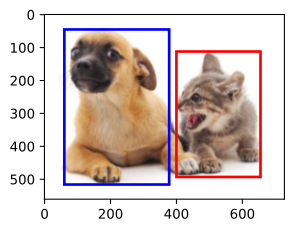
\includegraphics[width=0.55\linewidth]{Images/Congnghelienquan/output_bounding-box.png}
    \caption{Minh họa bài toán object detection với cơ chế bounding box \parencite{d2l_bounding_box}}
    \label{fig:object-detection-example}
\end{figure}

Các mô hình object detection thường được chia thành:

\begin{itemize}
    \item \textbf{One-stage detectors}: Thực hiện dự đoán trực tiếp vị trí bounding box và nhãn đối tượng trong một lần xử lý. Nhóm mô hình này thường có tốc độ nhanh, phù hợp với các bài toán yêu cầu xử lý thời gian thực như YOLO hoặc SSD.
    
    \item \textbf{Two-stage detectors}: Thực hiện theo hai bước, đầu tiên đề xuất các vùng có khả năng chứa đối tượng, sau đó phân loại đối tượng và tinh chỉnh bounding box cho từng vùng. Nhóm mô hình này thường có độ chính xác cao hơn nhưng tốc độ xử lý chậm hơn, ví dụ như R-CNN và Faster R-CNN.
\end{itemize}
%=========================
\subsubsection{YOLO}

YOLO (You Only Look Once) là mô hình object detection thuộc nhóm one-stage detector, được giới thiệu bởi Redmon et al. \parencite{redmon2016yolo}. Mô hình này được tối ưu cho các bài toán phát hiện đối tượng thời gian thực nhờ khả năng dự đoán vị trí và nhãn đối tượng chỉ trong một lần xử lý ảnh.

Khác với các mô hình two-stage detector cần đề xuất vùng trước khi phân loại, YOLO chia ảnh đầu vào thành các vùng lưới và trực tiếp dự đoán bounding box, confidence score và class probability cho các đối tượng xuất hiện trong ảnh. Cách tiếp cận này giúp YOLO có tốc độ xử lý nhanh, phù hợp với các hệ thống cần phản hồi gần như tức thời.

Về kiến trúc, YOLO thường gồm ba thành phần chính: backbone, neck và detection head. Backbone được sử dụng để trích xuất đặc trưng từ ảnh đầu vào, neck tổng hợp đặc trưng ở nhiều tầng khác nhau, còn detection head thực hiện dự đoán bounding box, class và confidence score cho từng đối tượng.

Trong hệ thống AI Shopping Assistant, YOLO có thể được sử dụng để phát hiện sản phẩm trong ảnh người dùng, xử lý nhiều đối tượng xuất hiện cùng lúc và hỗ trợ visual search nhanh. Ví dụ, khi người dùng tải lên một ảnh có chứa áo, giày hoặc túi xách, YOLO có thể xác định vùng chứa từng sản phẩm để hệ thống tiếp tục trích xuất đặc trưng hình ảnh và tìm kiếm các sản phẩm tương tự.

\begin{figure}[H]
    \centering
    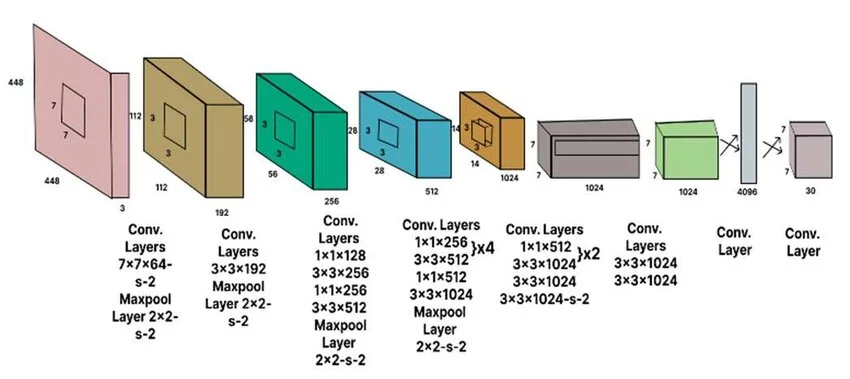
\includegraphics[width=0.95\linewidth]{Images/Congnghelienquan/yolo-architecture.png}
    \caption{Kiến trúc mô hình YOLO với pipeline one-stage detection từ backbone, neck đến detection head, thực hiện dự đoán bounding box và class probability trong một forward pass (nguồn: ResearchGate \parencite{researchgate_yolo_architecture})}
    \label{fig:yolo-architecture}
\end{figure}
\subsubsection{Faster R-CNN}

Faster R-CNN là mô hình object detection thuộc nhóm two-stage detector, được giới thiệu nhằm cải thiện tốc độ và độ chính xác so với các phiên bản R-CNN trước đó \textcite{ren2015fasterrcnn}. Khác với các mô hình one-stage detector dự đoán trực tiếp bounding box và class trong một lần xử lý, Faster R-CNN thực hiện phát hiện đối tượng theo hai giai đoạn.

Ở giai đoạn đầu, mô hình sử dụng Region Proposal Network (RPN) để sinh ra các vùng ứng viên có khả năng chứa đối tượng. Ở giai đoạn tiếp theo, các vùng ứng viên này được đưa vào mạng phân loại để xác định nhãn đối tượng và tinh chỉnh lại tọa độ bounding box. Cách tiếp cận hai giai đoạn giúp Faster R-CNN đạt độ chính xác cao trong việc phát hiện và định vị đối tượng.

Trong hệ thống AI Shopping Assistant, Faster R-CNN có thể được sử dụng để phát hiện và định vị sản phẩm trong ảnh người dùng, đặc biệt trong các trường hợp ảnh có nhiều đối tượng hoặc cần độ chính xác cao. Mô hình có thể hỗ trợ visual search bằng cách xác định vùng chứa sản phẩm, sau đó hệ thống sử dụng vùng ảnh này để trích xuất đặc trưng và truy xuất các sản phẩm tương tự.

Ưu điểm của Faster R-CNN là độ chính xác cao, khả năng định vị đối tượng tốt và phù hợp với các bài toán có nhiều đối tượng trong cùng một ảnh. Tuy nhiên, do kiến trúc gồm nhiều bước xử lý, mô hình này thường có tốc độ chậm hơn các mô hình one-stage như YOLO và yêu cầu tài nguyên tính toán cao hơn.
%=========================
\subsubsection{DETR}

DETR (DEtection TRansformer) là mô hình object detection dựa trên kiến trúc Transformer \textcite{carion2020detr}. Khác với các mô hình object detection truyền thống thường sử dụng anchor boxes hoặc các bước hậu xử lý như Non-Maximum Suppression (NMS), DETR xem bài toán phát hiện đối tượng như một bài toán dự đoán tập hợp đối tượng trong ảnh.

Kiến trúc của DETR gồm CNN backbone để trích xuất đặc trưng hình ảnh và Transformer encoder-decoder để mô hình hóa quan hệ giữa các vùng trong ảnh. Sau đó, mô hình dự đoán trực tiếp các đối tượng thông qua object queries, bao gồm nhãn đối tượng và tọa độ bounding box tương ứng. Cách tiếp cận này giúp DETR có kiến trúc end-to-end rõ ràng hơn so với nhiều pipeline detection truyền thống.

Trong hệ thống AI Shopping Assistant, DETR có thể được sử dụng để phát hiện sản phẩm trong ảnh người dùng, đặc biệt trong các trường hợp ảnh chứa nhiều đối tượng hoặc cần hiểu mối quan hệ giữa các vùng ảnh. Ví dụ, nếu người dùng tải lên một ảnh có nhiều sản phẩm như áo, túi xách và giày, DETR có thể xác định từng đối tượng để hệ thống tiếp tục xử lý visual search hoặc recommendation.

Ưu điểm của DETR là kiến trúc end-to-end, khả năng xử lý tốt bài toán nhiều đối tượng và giảm phụ thuộc vào các bước hậu xử lý phức tạp như anchor design hoặc NMS. Tuy nhiên, mô hình này thường có chi phí huấn luyện cao, yêu cầu tài nguyên tính toán lớn và có thể cần nhiều dữ liệu để đạt hiệu quả tốt trong thực tế.
%=========================
\subsubsection{So sánh các mô hình Object Detection}

\begin{table}[H]
\centering
\caption{So sánh các mô hình object detection theo kiến trúc, hiệu năng và mức độ phù hợp ứng dụng}
\label{tab:object-detection-models}
\begin{tabularx}{\linewidth}{@{}p{0.18\linewidth}X X X@{}}
\toprule
\textbf{Tiêu chí} & \textbf{YOLO} & \textbf{Faster R-CNN} & \textbf{DETR} \\
\midrule
Kiến trúc & One-stage CNN & Two-stage CNN & Transformer-based \\
Tốc độ inference & Rất cao & Trung bình & Trung bình \\
Độ chính xác & Cao & Rất cao & Cao \\
Khả năng realtime & Rất tốt & Hạn chế & Trung bình \\
Độ phức tạp & Thấp & Cao & Cao \\
Global context modeling & Trung bình & Trung bình & Rất tốt \\
Yêu cầu tài nguyên & Trung bình & Cao & Rất cao \\
Ứng dụng phù hợp & Real-time detection & High-precision tasks & Vision Transformer systems \\
\bottomrule
\end{tabularx}
\end{table}

\noindent
Trong hệ thống AI Shopping Assistant, YOLO được ưu tiên cho các tác vụ real-time detection, Faster R-CNN phù hợp với các bài toán yêu cầu độ chính xác cao, trong khi DETR đại diện cho hướng tiếp cận hiện đại dựa trên Transformer với khả năng modeling global context tốt hơn.
\subsection{Vector Databases}
Vector Database là hệ cơ sở dữ liệu được tối ưu cho việc lưu trữ và truy xuất vector embedding phục vụ semantic search và similarity search.

Trong hệ thống AI Shopping Assistant, vector database được sử dụng để:
\begin{itemize}
    \item Lưu trữ text embeddings và image embeddings
    \item Tìm kiếm sản phẩm tương tự
    \item Hỗ trợ multimodal retrieval
    \item Tăng tốc ANN search
\end{itemize}

Các vector database hiện đại thường hỗ trợ ANN indexing, metadata filtering và realtime retrieval.
\subsubsection{Pinecone}

Pinecone là vector database dạng managed cloud service được tối ưu cho các ứng dụng semantic search và retrieval \parencite{pinecone_docs}. Hệ thống này hỗ trợ realtime indexing, metadata filtering, hybrid search kết hợp dense và sparse vectors, cũng như ANN search trên tập dữ liệu vector có quy mô lớn.

Trong hệ thống AI Shopping Assistant, Pinecone có thể được sử dụng để lưu trữ text embeddings và image embeddings của sản phẩm, từ đó hỗ trợ semantic product search, recommendation retrieval và RAG retrieval pipeline. Khi người dùng nhập truy vấn hoặc tải lên hình ảnh, hệ thống có thể chuyển dữ liệu đầu vào thành embedding và truy xuất các sản phẩm có độ tương đồng cao trong Pinecone.

Ưu điểm của Pinecone là dễ triển khai, có khả năng mở rộng tốt và giảm gánh nặng quản trị hạ tầng vì được cung cấp dưới dạng managed service. Tuy nhiên, hạn chế của Pinecone là chi phí có thể tăng khi dữ liệu lớn hoặc số lượng truy vấn cao, đồng thời hệ thống cũng phụ thuộc vào cloud service bên ngoài.

\begin{figure}[H]
    \centering
    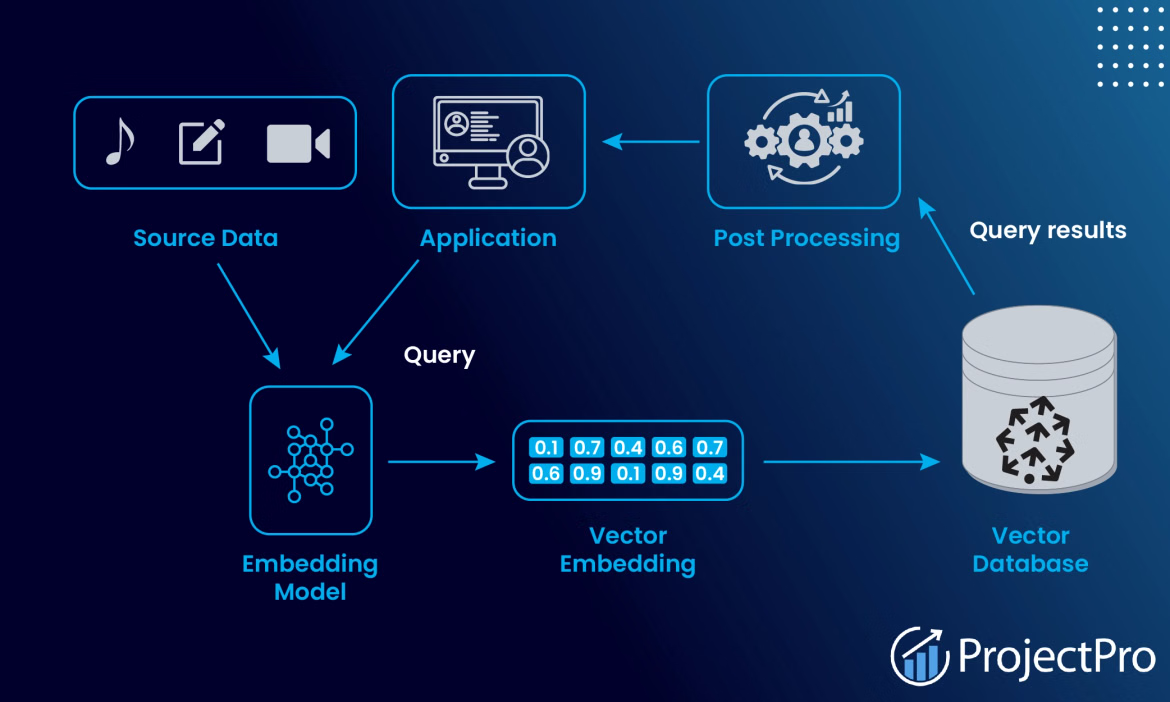
\includegraphics[width=0.7\linewidth]{Images/Congnghelienquan/pinecone-vector-indexing.png}
    \caption{Kiến trúc Pinecone Vector Database minh họa pipeline indexing và similarity search (nguồn: ProjectPro) \parencite{projectpro2026pinecone}}
    \label{fig:pinecone-vector-indexing}
\end{figure}
\subsubsection{Qdrant}

Qdrant là vector database mã nguồn mở được tối ưu cho similarity search và các ứng dụng AI \parencite{qdrant_docs}. Hệ thống này hỗ trợ realtime vector retrieval, payload filtering và hybrid search, giúp kết hợp tìm kiếm vector với các điều kiện lọc dựa trên metadata.

Qdrant sử dụng HNSW (Hierarchical Navigable Small World) để tăng tốc ANN search trên tập dữ liệu lớn. Nhờ đó, hệ thống có thể truy xuất các vector tương đồng với tốc độ cao mà không cần duyệt toàn bộ dữ liệu.

\begin{figure}[H]
    \centering
    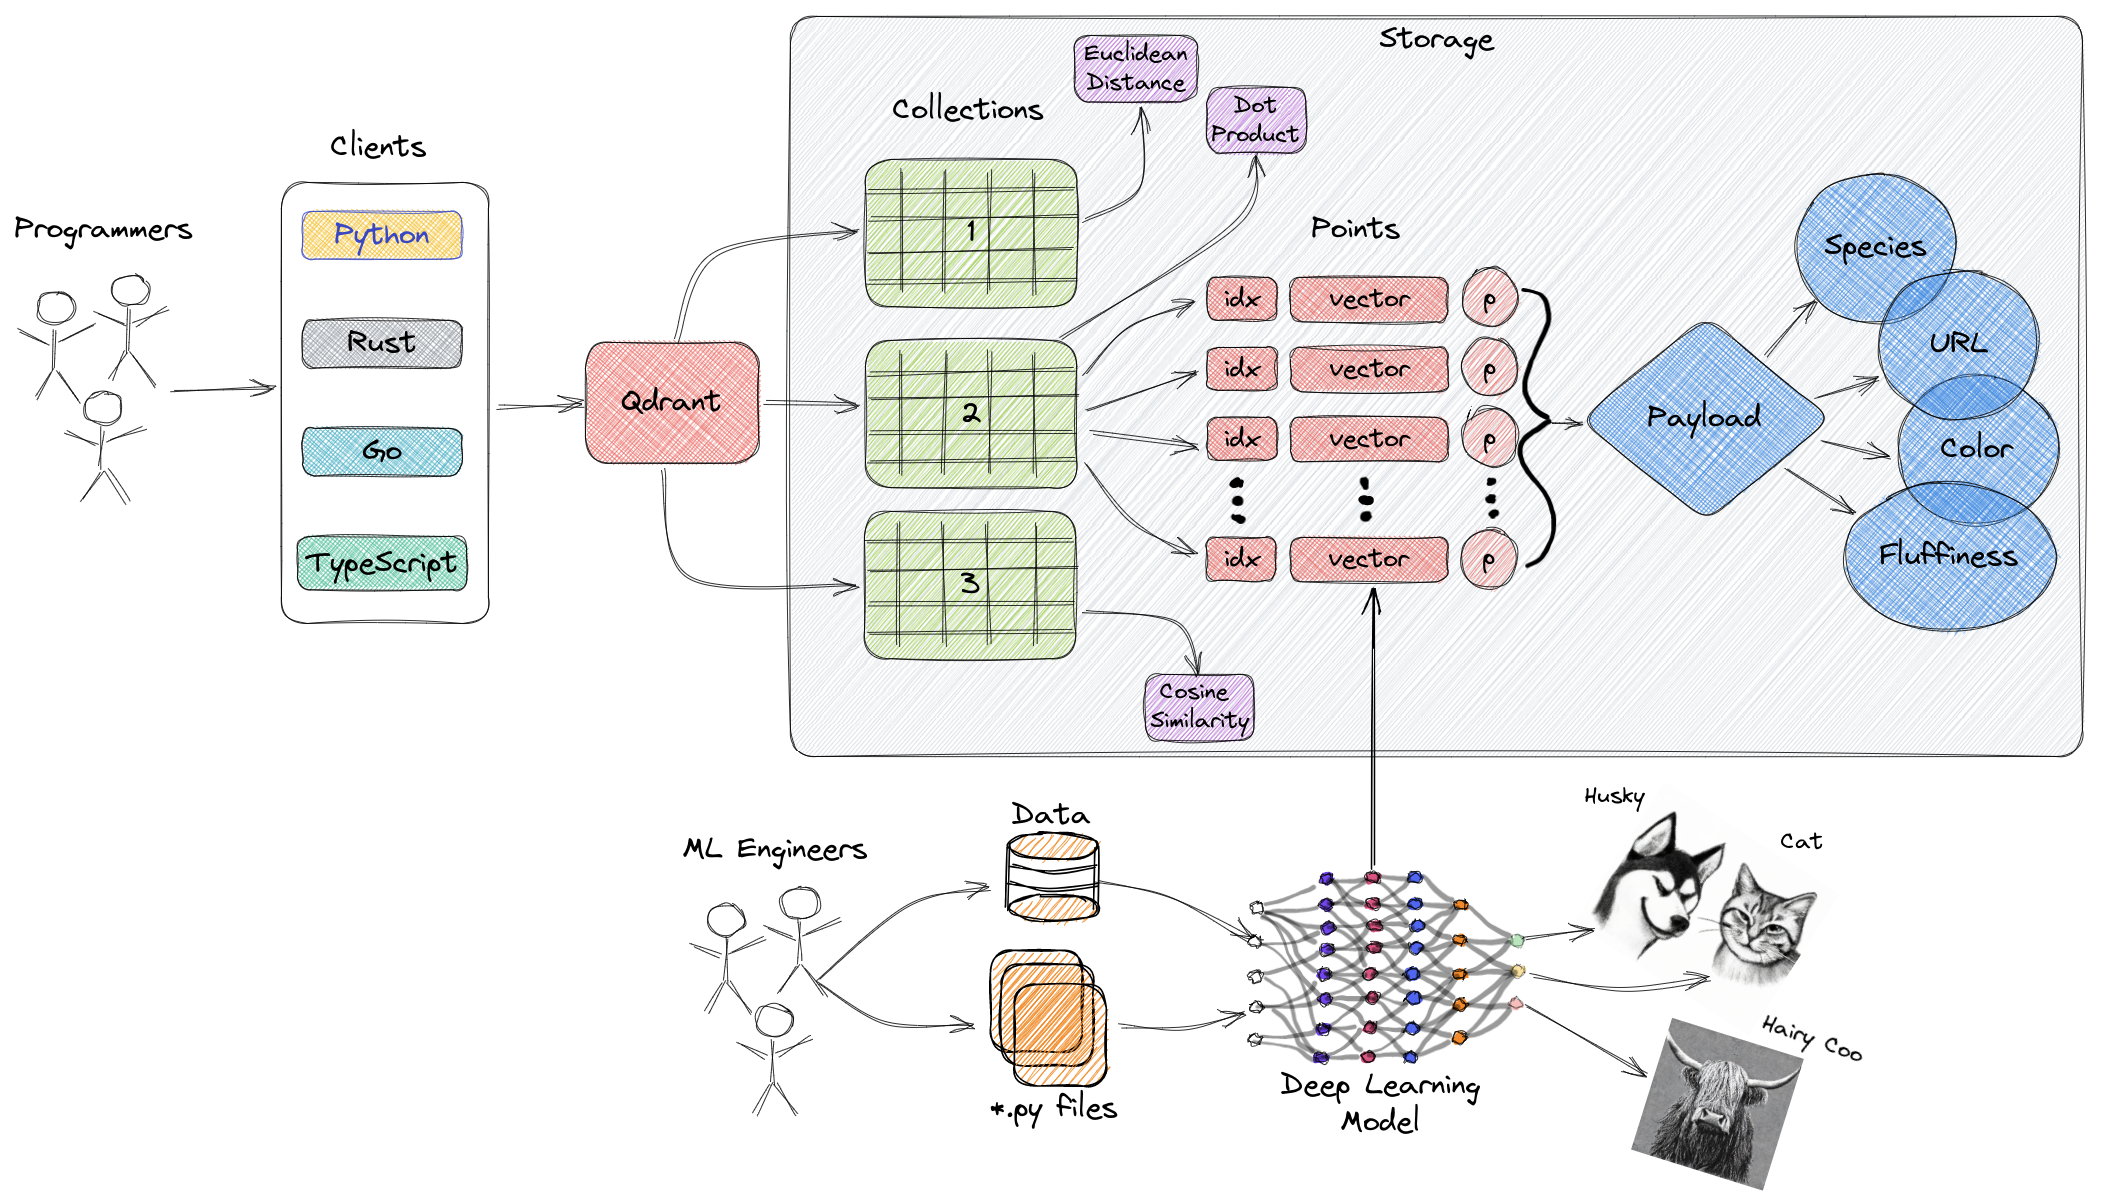
\includegraphics[width=0.9\linewidth]{Images/Congnghelienquan/qdrant_overview_high_level.png}
    \caption{Kiến trúc Qdrant Vector Database với core vector engine, storage layer và filtering system, hỗ trợ semantic search và hybrid search trong các ứng dụng AI hiện đại \parencite{qdrant_overview}}
    \label{fig:qdrant-vector-database}
\end{figure}

Một số tính năng nổi bật của Qdrant bao gồm khả năng lưu trữ vector embedding, payload filtering, hybrid search, REST API và gRPC support. Các tính năng này giúp Qdrant phù hợp với những hệ thống cần truy xuất dữ liệu nhanh, có điều kiện lọc linh hoạt và dễ tích hợp với backend service.

Trong hệ thống AI Shopping Assistant, Qdrant có thể được sử dụng làm semantic search engine, product recommendation engine, multimodal retrieval system hoặc self-hosted vector infrastructure. Hệ thống có thể lưu trữ embedding của sản phẩm, văn bản và hình ảnh để phục vụ tìm kiếm ngữ nghĩa, tìm kiếm bằng hình ảnh và gợi ý sản phẩm.

Ưu điểm của Qdrant là dễ self-host, hỗ trợ metadata filtering mạnh và có hiệu năng retrieval tốt. Tuy nhiên, khi triển khai ở quy mô lớn, hệ thống cần tự quản lý infrastructure và việc distributed scaling có thể phức tạp hơn so với các managed vector database service.
\subsubsection{Milvus}

Milvus là vector database mã nguồn mở được phát triển cho các ứng dụng AI quy mô lớn \parencite{milvus_docs}. Hệ thống này hỗ trợ nhiều thuật toán ANN indexing như HNSW, IVF, Product Quantization (PQ) và DiskANN, giúp tối ưu quá trình tìm kiếm vector trên các tập dữ liệu lớn.

Milvus được thiết kế để phục vụ các bài toán billion-scale vector search, distributed deployment, GPU acceleration và cloud-native architecture. Nhờ đó, Milvus phù hợp với các hệ thống cần xử lý lượng lớn embedding và yêu cầu khả năng truy xuất nhanh trong môi trường production.

\begin{figure}[H]
    \centering
    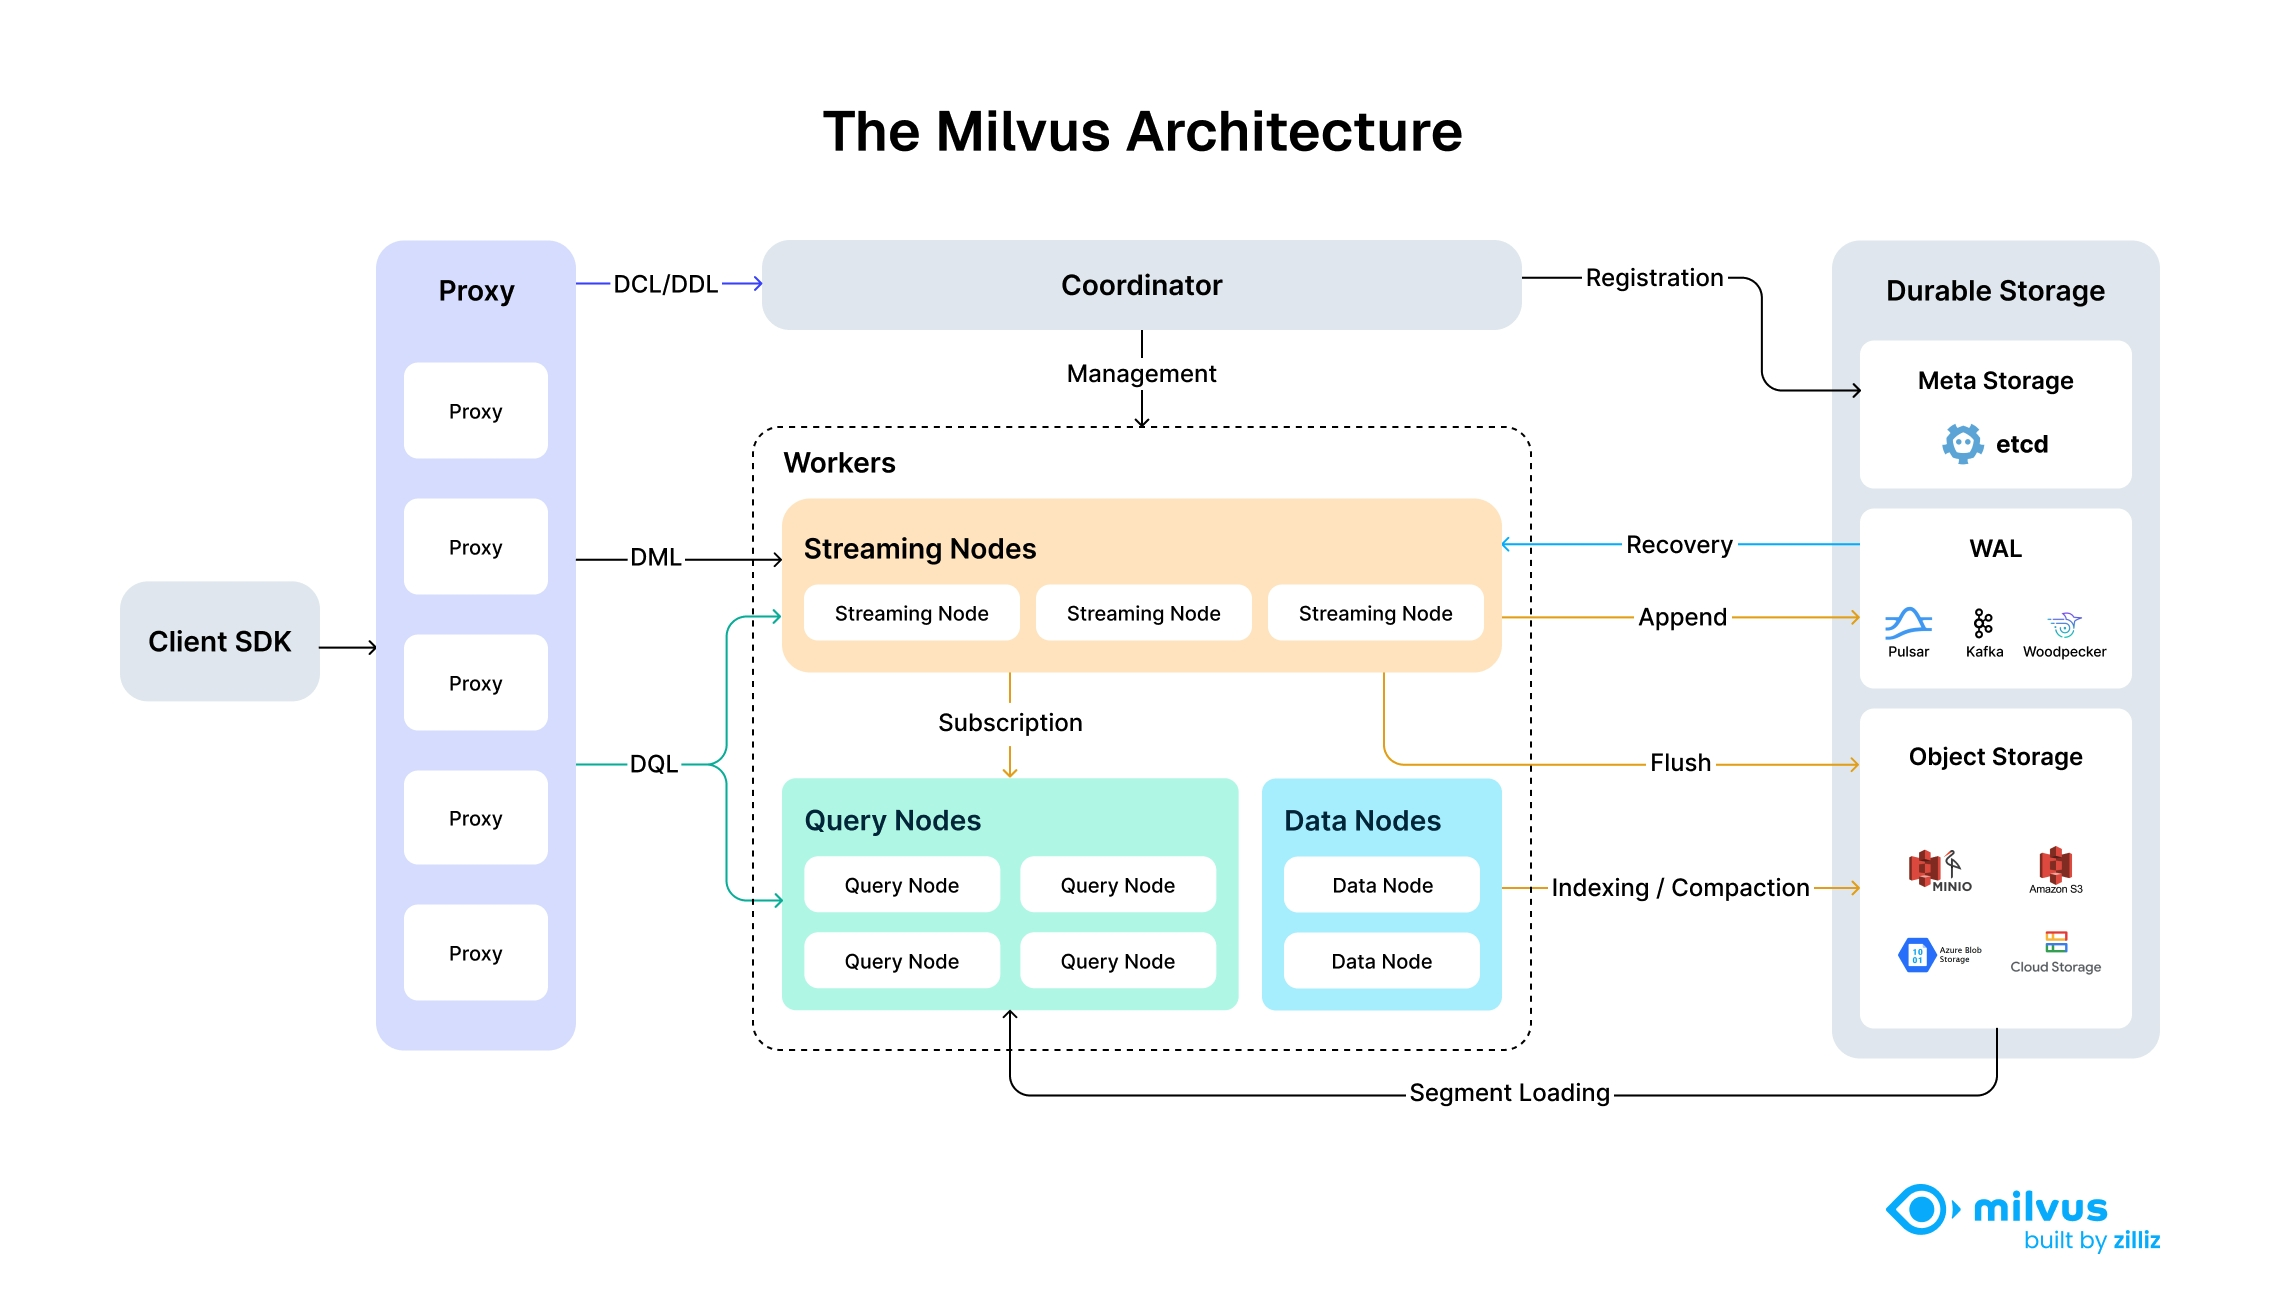
\includegraphics[width=1\linewidth]{Images/Congnghelienquan/milvus_architecture.png}
    \caption{Kiến trúc Milvus Vector Database với các lớp Access Layer, Coordinator, Worker Nodes và Storage, minh họa pipeline indexing và similarity search trong hệ thống phân tán \parencite{milvus_architecture_overview}}
    \label{fig:milvus-vector-indexing}
\end{figure}

Trong hệ thống AI Shopping Assistant, Milvus có thể được sử dụng cho large-scale product retrieval, high-throughput semantic search và multimodal vector indexing. Cụ thể, hệ thống có thể lưu trữ embedding của văn bản, hình ảnh và metadata sản phẩm để phục vụ tìm kiếm ngữ nghĩa, tìm kiếm bằng hình ảnh và gợi ý sản phẩm.

Ưu điểm của Milvus là khả năng mở rộng rất lớn, hỗ trợ GPU acceleration và phù hợp với các production AI systems. Tuy nhiên, hạn chế của Milvus là quá trình triển khai phức tạp hơn so với các managed vector database, đồng thời yêu cầu tài nguyên hệ thống cao khi vận hành ở quy mô lớn.

\subsubsection{So sánh Vector Database}

\begin{table}[H]
\centering
\caption{So sánh các vector database phổ biến cho hệ thống AI}
\label{tab:vector-db-comparison}
\renewcommand{\arraystretch}{1.3}

\begin{tabularx}{\linewidth}{
@{}
p{0.20\linewidth}
p{0.24\linewidth}
p{0.24\linewidth}
p{0.24\linewidth}
@{}
}
\toprule

\textbf{Tiêu chí} &
\textbf{Pinecone} &
\textbf{Qdrant} &
\textbf{Milvus} \\

\midrule

Loại &
Managed cloud service &
Open-source &
Open-source \\

Khả năng mở rộng &
Rất cao &
Cao &
Rất cao \\

Triển khai &
Dễ &
Trung bình &
Phức tạp \\

ANN indexing &
Có &
Có &
Có \\

Metadata filtering &
Tốt &
Rất tốt &
Tốt \\

GPU support &
Hạn chế &
Không chính thức &
Có \\

Distributed architecture &
Managed infrastructure &
Có &
Rất mạnh \\

Phù hợp &
Startup, SaaS &
Self-hosted AI systems &
Large-scale AI systems \\

\bottomrule
\end{tabularx}

\end{table}
\subsection{AI Agent Frameworks}

AI Agent frameworks là nhóm công cụ hỗ trợ xây dựng các hệ thống dựa trên LLM, cho phép mô hình có khả năng lập kế hoạch, gọi công cụ, duy trì trạng thái hội thoại và thực thi workflow phức tạp. Trong các hệ thống hiện đại như AI Shopping Assistant, các framework này đóng vai trò trung tâm trong việc điều phối truy vấn người dùng, tích hợp retrieval và tương tác với các dịch vụ bên ngoài.

%=========================
\subsubsection{LangChain}

LangChain là một framework phổ biến để xây dựng ứng dụng dựa trên LLMs, cung cấp các abstraction cho prompt management, memory, chains và tool calling \parencite{langchain2024docs}.

Các thành phần chính:
\begin{itemize}
    \item LLM wrappers: tích hợp nhiều mô hình ngôn ngữ
    \item Chains: chuỗi xử lý nhiều bước
    \item Memory: lưu trạng thái hội thoại
    \item Tools: tích hợp API và external services
\end{itemize}

LangChain phù hợp cho các ứng dụng prototype nhanh, chatbot và hệ thống RAG đơn giản. Tuy nhiên, khi workflow trở nên phức tạp và có nhiều trạng thái điều kiện, việc quản lý luồng có thể trở nên khó kiểm soát.

% % (Gợi ý hình 1)
% \begin{figure}[H]
%     \centering
%     \includegraphics[width=0.85\linewidth]{Images/ai-agents/langchain-architecture.png}
%     \caption{Kiến trúc tổng quan của LangChain với các thành phần LLM, Chains, Memory và Tools}
%     \label{fig:langchain-architecture}
% \end{figure}

%=========================
\subsubsection{LangGraph}

LangGraph là một extension của LangChain, được thiết kế để hỗ trợ stateful workflows dưới dạng directed graph \parencite{langgraph2024docs}. Khác với mô hình chain tuyến tính, LangGraph cho phép xây dựng các agent có khả năng:

\begin{itemize}
    \item Quản lý trạng thái phức tạp (stateful execution)
    \item Rẽ nhánh logic (conditional routing)
    \item Loop giữa các node trong graph
\end{itemize}

Điều này đặc biệt phù hợp với các hệ thống AI agent thực tế như shopping assistant, nơi truy vấn có thể đi qua nhiều bước: hiểu query → retrieval → rerank → phản hồi → tool calling lại nếu cần.

% (Gợi ý hình 2)
% \begin{figure}[H]
%     \centering
%     \includegraphics[width=0.85\linewidth]{Images/ai-agents/langgraph-workflow.png}
%     \caption{Mô hình graph-based workflow của LangGraph với các node xử lý trạng thái}
%     \label{fig:langgraph-workflow}
% \end{figure}

%=========================
\subsubsection{LlamaIndex}

LlamaIndex là framework tập trung vào xây dựng hệ thống Retrieval-Augmented Generation (RAG), giúp kết nối dữ liệu riêng với LLM \parencite{llamaindex2024docs}.

Các chức năng chính:
\begin{itemize}
    \item Data ingestion: đọc dữ liệu từ nhiều nguồn (PDF, database, API)
    \item Indexing: xây dựng vector index
    \item Query engine: truy vấn semantic search
    \item Integration với LLMs
\end{itemize}

Trong hệ thống AI Shopping Assistant, LlamaIndex thường được sử dụng cho:
\begin{itemize}
    \item Tìm kiếm sản phẩm từ database nội bộ
    \item Semantic retrieval cho mô tả sản phẩm
    \item Hỗ trợ hybrid search (text + metadata)
\end{itemize}

% % (Gợi ý hình 3 - optional nhưng nên có 1 hình tổng)
% \begin{figure}[H]
%     \centering
%     \includegraphics[width=0.85\linewidth]{Images/ai-agents/llamaindex-rag.png}
%     \caption{Pipeline RAG của LlamaIndex từ dữ liệu đầu vào đến truy vấn LLM}
%     \label{fig:llamaindex-rag}
% \end{figure}

%=========================
\subsubsection{So sánh AI agent frameworks}

\begin{table}[H]
\centering
\caption{So sánh các AI agent frameworks trong xây dựng hệ thống LLM-based applications}
\label{tab:ai-agent-frameworks}
\renewcommand{\arraystretch}{1.3}
\begin{tabularx}{\linewidth}{@{}p{0.18\linewidth}X X X@{}}
\toprule
\textbf{Tiêu chí} & \textbf{LangChain} & \textbf{LangGraph} & \textbf{LlamaIndex} \\
\midrule
Mục tiêu chính 
& Xây dựng ứng dụng LLM tổng quát và tích hợp công cụ 
& Xây dựng agent workflow có trạng thái và luồng xử lý phức tạp 
& Xây dựng hệ thống indexing, retrieval và RAG \\

Kiến trúc 
& Chain-based 
& Graph-based state machine 
& Index-based retrieval pipeline \\

Quản lý trạng thái 
& Cơ bản 
& Tốt, phù hợp các workflow nhiều bước 
& Trung bình \\

Điều phối workflow 
& Trung bình 
& Mạnh, hỗ trợ luồng xử lý phân nhánh và lặp 
& Trung bình \\

Khả năng sử dụng công cụ 
& Có hỗ trợ tool calling 
& Mạnh, phù hợp agent cần phối hợp nhiều công cụ 
& Có hỗ trợ, nhưng trọng tâm là retrieval \\

Khả năng RAG 
& Có hỗ trợ 
& Có thể tích hợp vào workflow của agent 
& Mạnh, tập trung vào indexing và retrieval \\

Độ phức tạp triển khai 
& Trung bình 
& Cao hơn do cần thiết kế graph và state 
& Trung bình \\

Ứng dụng phù hợp 
& Chatbot, prototype, LLM app tổng quát 
& AI agent nhiều bước, workflow có trạng thái, tác vụ cần điều phối 
& Search engine, knowledge base, RAG system \\
\bottomrule
\end{tabularx}
\end{table}

\noindent
Nhìn chung, LangChain phù hợp với các ứng dụng LLM tổng quát và các hệ thống cần tích hợp nhanh với nhiều công cụ. LangGraph phù hợp hơn với các bài toán agent có nhiều bước xử lý, cần quản lý trạng thái và điều phối luồng thực thi phức tạp. Trong khi đó, LlamaIndex có thế mạnh ở các hệ thống tập trung vào indexing, retrieval và RAG. Vì vậy, việc lựa chọn framework phụ thuộc vào trọng tâm của hệ thống: hội thoại tổng quát, workflow agent hay truy xuất tri thức.

% \subsection{Các công nghệ liên quan đến RAG và hệ thống LLM}

% Các kỹ thuật RAG và hệ thống dựa trên LLM giúp nâng cao hiệu quả truy xuất thông tin và xử lý ngôn ngữ tự nhiên bằng cách kết hợp mô hình ngôn ngữ với nguồn tri thức bên ngoài, cơ chế suy luận và khả năng sử dụng công cụ.
% %=========================
% \subsubsection{Conversational RAG}

% Conversational RAG là một biến thể của RAG được thiết kế để xử lý các tình huống hội thoại nhiều lượt. Khác với mô hình RAG truyền thống chỉ xử lý từng truy vấn riêng lẻ, Conversational RAG tận dụng ngữ cảnh từ lịch sử hội thoại để cải thiện quá trình truy xuất thông tin.

% Đặc điểm chính:
% \begin{itemize}
%     \item Hỗ trợ hội thoại nhiều lượt (multi-turn conversation)
%     \item Tận dụng lịch sử hội thoại để cải thiện độ liên quan của kết quả truy xuất
%     \item Giảm tình trạng mơ hồ trong các truy vấn ngắn hoặc thiếu ngữ cảnh
% \end{itemize}

% %=========================
% \subsubsection{Kỹ thuật viết lại truy vấn (Query Rewriting)}

% Kỹ thuật viết lại truy vấn là phương pháp chuyển đổi câu truy vấn ban đầu thành dạng tối ưu hơn nhằm nâng cao hiệu quả truy xuất thông tin.

% Mục tiêu của kỹ thuật này:
% \begin{itemize}
%     \item Tăng độ rõ ràng và đầy đủ ngữ nghĩa của truy vấn
%     \item Bổ sung thông tin ngữ cảnh bị thiếu
%     \item Giảm sự mơ hồ trong các truy vấn ngắn
% \end{itemize}

% Kỹ thuật này thường được sử dụng trong các hệ thống tìm kiếm và truy xuất thông tin hiện đại.

% %=========================
% \subsubsection{Gọi công cụ (Tool Calling)}

% Tool Calling là cơ chế cho phép mô hình ngôn ngữ lớn tương tác với các hệ thống bên ngoài thông qua việc sinh ra các đầu ra có cấu trúc để kích hoạt các hàm hoặc API tương ứng.
% Các loại công cụ phổ biến:
% \begin{itemize}
%     \item Công cụ truy vấn cơ sở dữ liệu vector
%     \item API truy xuất dữ liệu sản phẩm
%     \item Công cụ tìm kiếm thông tin
%     \item Các dịch vụ lọc hoặc xử lý dữ liệu
% \end{itemize}

% Cơ chế này giúp mở rộng khả năng của LLM từ việc sinh văn bản sang thực hiện hành động.

% %=========================
% \subsubsection{Cơ chế bộ nhớ trong hệ thống LLM}

% Cơ chế bộ nhớ  trong các hệ thống LLM cho phép lưu trữ và sử dụng lại thông tin từ các tương tác trước đó nhằm duy trì tính liên tục của ngữ cảnh.

% Các dạng bộ nhớ phổ biến:
% \begin{itemize}
%     \item Bộ nhớ ngắn hạn: lưu trữ ngữ cảnh hội thoại gần nhất
%     \item Bộ nhớ dài hạn: lưu trữ thông tin người dùng hoặc tri thức lâu dài
%     \item Bộ nhớ tóm tắt: nén nội dung hội thoại dài thành dạng ngắn gọn
% \end{itemize}

% Cơ chế này giúp cải thiện tính nhất quán trong các hệ thống hội thoại dài.

% %=========================
% \subsubsection{Kỹ thuật suy luận nhiều bước}

% Các kỹ thuật suy luận nhiều bước cho phép mô hình ngôn ngữ thực hiện quá trình xử lý theo từng bước thay vì đưa ra câu trả lời trực tiếp.

% Một số phương pháp phổ biến:
% \begin{itemize}
%     \item Chain-of-Thought (suy luận theo chuỗi)
%     \item Phân rã bài toán thành các bước nhỏ
%     \item Suy luận từng bước có kiểm soát
% \end{itemize}

% Các kỹ thuật này giúp cải thiện khả năng giải quyết các truy vấn phức tạp.

% %=========================
% \subsubsection{Hệ thống tác tử dựa trên LLM}

% Hệ thống tác tử  là các hệ thống mở rộng từ mô hình ngôn ngữ lớn, cho phép mô hình không chỉ sinh văn bản mà còn đưa ra quyết định và thực hiện hành động trong môi trường bên ngoài.

% Đặc điểm:
% \begin{itemize}
%     \item Kết hợp giữa suy luận và hành động
%     \item Có khả năng lựa chọn công cụ phù hợp
%     \item Thực hiện xử lý theo nhiều bước lặp lại
% \end{itemize}

% Các hệ thống này đánh dấu sự chuyển đổi từ mô hình sinh văn bản thụ động sang mô hình giải quyết vấn đề chủ động.

% %=========================
% \begin{table}[H]
% \centering
% \caption{RAG và hệ thống LLM}
% \label{tab:rag_llm_vietnamese}
% \begin{tabularx}{\linewidth}{@{}p{0.35\linewidth}X@{}}
% \toprule
% \textbf{Công nghệ} & \textbf{Mô tả} \\
% \midrule
% Conversational RAG & Mở rộng RAG cho hội thoại nhiều lượt dựa trên ngữ cảnh \\
% Query Rewriting & Kỹ thuật tối ưu hóa truy vấn nhằm cải thiện chất lượng truy xuất \\
% Tool Calling & Cơ chế cho phép LLM gọi các hàm hoặc API bên ngoài \\
% Cơ chế bộ nhớ & Lưu trữ và tái sử dụng thông tin hội thoại trong LLM \\
% Suy luận nhiều bước & Các phương pháp giúp mô hình giải quyết bài toán phức tạp theo từng bước \\
% Hệ thống tác tử LLM & Mô hình kết hợp suy luận, lựa chọn hành động và sử dụng công cụ \\
% \bottomrule
% \end{tabularx}
% \end{table}
